%%%%%%%%%%%%%%%%%%%%%%%%%%%%%%%%%%%%%%%%%%%%%%%%%%%%%%%%%%%%%%%%%%%%%%%%%%%%%%%%
%2345678901234567890123456789012345678901234567890123456789012345678901234567890
%        1         2         3         4         5         6         7         8

\documentclass{ieeetrans}   % Comment this line out if you need a4paper

%\documentclass[a4paper, 10pt, conference]{ieeeconf}      % Use this line for a4 paper

\IEEEoverridecommandlockouts                              % This command is only needed if 
                                                          % you want to use the \thanks command

%\overrideIEEEmargins                                      % Needed to meet printer requirements.

\usepackage{pgfplots}
\pgfplotsset{compat=1.16}
\pdfobjcompresslevel=0

%In case you encounter the following error:
%Error 1010 The PDF file may be corrupt (unable to open PDF file) OR
%Error 1000 An error occurred while parsing a contents stream. Unable to analyze the PDF file.
%This is a known problem with pdfLaTeX conversion filter. The file cannot be opened with acrobat reader
%Please use one of the alternatives below to circumvent this error by uncommenting one or the other
%\pdfobjcompresslevel=0
%\pdfminorversion=4

% See the \addtolength command later in the file to balance the column lengths
% on the last page of the document

% The following packages can be found on http:\\www.ctan.org
\usepackage{cite}
\usepackage{url}
\usepackage{graphics} % for pdf, bitmapped graphics files
\usepackage{epsfig} % for postscript graphics files
\usepackage{mathptmx} % assumes new font selection scheme installed
\usepackage{mathrsfs}
\DeclareMathAlphabet{\mathcal}{OMS}{cmsy}{m}{n}
\usepackage{cuted}

%\usepackage{times} % assumes new font selection scheme installed
\usepackage{setspace}
\usepackage{amssymb,amsmath,amsfonts}
%\usepackage{mathrsfs}
%\usepackage{amsthm}
\usepackage{ntheorem}
\usepackage{booktabs}
\usepackage{makecell}
\let\labelindent\relax
\usepackage{enumitem}
\usepackage{mathtools}
\usepackage{esvect}

\usetikzlibrary{circuits}

\usetikzlibrary{intersections} 

\usetikzlibrary{scopes, arrows, fadings, patterns}

\usetikzlibrary{%
	decorations.pathreplacing,%
	decorations.pathmorphing%
}

\usetikzlibrary{positioning}

\usepackage{bm}
\usepackage{tikz}
\usepackage{pgfplots}
\usepackage{algorithm,algorithmic}  
%\pgfplotsset{compat=1.6}
\usepackage{multirow}

\renewcommand{\labelenumi}{(\arabic{enumi})} % change enumerate env to (1)(2)(3)


\newcommand{\Pb}{{\mathbb{P}}}
\newcommand{\Eb}{{\mathbb{E}}}
\newcommand{\Rb}{{\mathbb{R}}}
\newcommand{\Cb}{{\mathbb{C}}}
\newcommand{\Ib}{{\mathbb{I}}}
\newcommand{\Zb}{{\mathbb{Z}}}

\newcommand{\Fs}{{\mathscr{F}}} % filiteration
\newcommand{\Bs}{{\mathscr{B}}} % Borel set
\newcommand{\Es}{{\mathscr{E}}}


\newcommand{\Ec}{{\mathcal{E}}} %graph vertex edge
\newcommand{\Gc}{{\mathcal{G}}}
\newcommand{\Vc}{{\mathcal{V}}}


\newcommand{\Fc}{{\mathcal{F}}}
\newcommand{\Pc}{{\mathcal{P}}}

\newcommand{\Qc}{{\mathcal{Q}}} 
\newcommand{\Ac}{{\mathcal{A}}}
\newcommand{\Cc}{{\mathcal{C}}}
\newcommand{\Ic}{{\mathcal{I}}}
\newcommand{\Rc}{{\mathcal{R}}}
\newcommand{\Uc}{{\mathcal{U}}}
\newcommand{\Tc}{{\mathcal{T}}}
\newcommand{\Sc}{{\mathcal{S}}}
\newcommand{\Oc}{{\mathcal{O}}}
\newcommand{\Mc}{{\mathcal{M}}}
\newcommand{\Nc}{{\mathcal{N}}}
\newcommand{\Wc}{{\mathcal{W}}}
\newcommand{\Lc}{{\mathcal{L}}}
\newcommand{\Hc}{{\mathcal{H}}}
\newcommand{\Xc}{{\mathcal{X}}}
\newcommand{\Yc}{{\mathcal{Y}}}

\newcommand{\Ss}{{\mathscr{S}}}

\newcommand{\Oi}{{\tilde{O}_i}}
\newcommand{\Gi}{{\tilde{G}_i}}
\newcommand{\Si}{{\tilde{S}_i}}

\newcommand{\ra}{{\rightarrow}}
\newcommand{\ift}{{\infty}}
\newcommand{\ls}{\text{ls}}
\newcommand{\re}{\text{true}}
\DeclareMathOperator{\rs}{{rowspan}}
\DeclareMathOperator{\rank}{{rank}}
\DeclareMathOperator{\sgn}{{sgn}}
\DeclareMathOperator{\diag}{{diag}}


\theorembodyfont{\normalfont}
\newtheorem{proposition}{\textbf{Proposition}}
\newtheorem{lemma}{\textbf{Lemma}}
\newtheorem{theorem}{\textbf{Theorem}}
\newtheorem{remark}{\textbf{Remark}}
\newtheorem{assumption}{\textbf{Assumption}}
\newtheorem{corollary}{\textbf{Corollary}}
\newtheorem{conjecture}{\textbf{Conjecture}}
\newtheorem{definition}{\textbf{Definition}}
\newtheorem{problem}{\textbf{Problem}}
%\newtheorem{proposition}{Proposition}
\newtheorem*{proof}{\textbf{Proof}}

\title{\LARGE \bf Low Complexity Secure State Estimation Design}


\author{Zishuo Li and Yilin Mo% <-this % stops a space
%\thanks{*This work was supported by }% <-this % stops a space
\thanks{Zishuo Li and Yilin Mo are with the Department
	of Automation, Tsinghua University, Beijing, China, e-mail: 
	lizs19@mails.tsinghua.edu.cn, ylmo@mail.tsinghua.edu.cn. }%
}


\begin{document}



\maketitle
%\thispagestyle{empty}
%\pagestyle{empty}


%%%%%%%%%%%%%%%%%%%%%%%%%%%%%%%%%%%%%%%%%%%%%%%%%%%%%%%%%%%%%%%%%%%%%%%%%%%%%%%%
\begin{abstract}
We consider the problem of estimating the state of a time-invariant linear Gaussian system in the presence of integrity attacks. The attacker can compromise $p$ out of $m$ sensors, the set of which is unknown to the system operator, and manipulate the measurements arbitrarily. Under the assumption that all the eigenvalues of system matrix $A$ have geometric multiplicity 1, we propose a secure estimation scheme that is resilient to integrity attack as long as the system is $2p$-sparse observable, which achieves the fundamental limit of secure state recovery. In the absence of attack, the proposed estimation coincides with Kalman estimation with a certain probability that can be adjusted to balance between performance with and without attack. Furthermore, our proposed estimator is computational efficient during the security condition checking in the designing phase and during the estimation computing in the online operating phase. A numerical example is provided to corroborate the results and illustrate the performance of the proposed estimator.


\end{abstract}


%%%%%%%%%%%%%%%%%%%%%%%%%%%%%%%%%%%%%%%%%%%%%%%%%%%%%%%%%%%%%%%%%%%%%%%%%%%%%%%%
\section{Introduction}
Cyber-Physical System (CPS) and Internet of Things (IoT) are playing an increasingly important role in critical infrastructures and everyday life. 
The related area of CPS and IoT continues to emerge and expand as costs drop and the confluence of sensors, platforms and networks increases\cite{2018DHS_report}.
Simultaneously, the cyber-security risks and attack surfaces are also increasing \cite{cardenas2008research} since CPS relies on remote sensing devices, communication channels, and spatially distributed processors, which are prone to failures under cyber attacks on the data acquisition and communication channels.
The unintentional faults or malicious attacks could cause severe system damage, economic loss, and environmental degradation, e.g., the Stuxnet launched on Iran’s nuclear facilities\cite{STUXNET}, power blackouts in Brazil \cite{samba_stop}, and Ukraine \cite{Ukraine_Blackout}, etc. The research community has recognized the importance of CPS security, especially the design of secure detection, estimation, and control strategy\cite{cardenas2009challenges}. 
%North America and Europe \cite{2003_blackout},

%The efforts fall into two major categories based on how the physical plant is modeled: 1) steady-state estimation (no dynamics) and 2) linear time invariant dynamics. In both categories the malicious attacker is assumed to corrupt a subset of sensors by manipulating the measurements, and the system operator intend to recover the system state based on the partly corrupted measurements.


%For the design of state estimators, Teixeira et al.~\cite{teixeira2010cyber} analyzed the effects of possible deceptions attacks for state
%estimators and proposed some policies to design deception attacks for both linear and nonlinear state estimation. Qi et al.~\cite{qi2015event}
%considered the event-based attack strategy against remote state estimation. Recently, Mo and Sinopoli~\cite{mo2015} proposed an estimator that
%has minimum mean square error against the worst-case attacks. However, the problem of designing a secure state estimator for a dynamic system
%is much more challenging because the bias injected by an adversary can accumulate in the dynamic state estimation and give rise to a large or
%even unbounded estimation error~\cite{moscs10security, mo2016}.


%To overcome the problem of bias accumulation in the dynamic state estimation, 

Recently, substantial research efforts have been devoted to secure state estimation against malicious sensors.
One of the research paths is the finite horizon approach, where only measurements in a finite time-window are considered when recovering the system state. 
The problem is combinatorial in nature since searching for the corrupted sensors involves minimizing the $\ell_0$ norm \cite{FawziTAC2014}, which is an NP problem.
Fawzi et al.~\cite{FawziTAC2014} propose an algorithm using its convex relaxation, i.e., $\ell_1$ optimization, to solve the problem in the absence of noise. 
Similarly, Shoukry and Tabuada \cite{ShoukryTAC2016} adopt a $2$-norm batch optimization approach to solve the state estimation problem.
Shoukry et al.~\cite{Shoukry2017} propose an algorithm in the presence of noise by searching for reliable sensors using consistency check, and the searching complexity is reduced based on Satisfiability Modulo Theory.
In addition to searching for reliable sensors, Guo et al. \cite{guoTSP2019} aim at locating compromised sensors by a Gaussian-mixture-model-based detection mechanism. The estimator fuses the measurements based on the belief given by the detection algorithm. 
However, in these works, the sensory data out of the time window are discarded, which may cause performance degradation and estimation delay.


Another solution is the switch estimator\cite{yorie}\cite{luTAC2019} where multiple estimates are maintained based on measurements from different subsets of sensors, and the system operator switches between these estimates based on the evaluation of their reliability by consistency checking or malicious detection algorithms. However, to guarantee that there is an estimate that does not take measurements from corrupted sensors, the number of alternative estimates is combinatorial. Maintaining these estimates may incur heavy computation and storage burden of the devices and increase the complexity of selecting reliable estimates.

In view of these problems, Liu et al. \cite{liuxinghua-TAC2020} design local estimators whose weighted sum coincides with the Kalman estimate with a certain probability in the absence of attack. The local estimates are fused securely by a quadratic programming problem with an $\ell_1$ term to handle the sparse outliers. 


Even though there are efficient algorithms computing the estimation by introducing $\ell_1$ relaxation, the design of the secure state estimation is still computational challenging. For secure state recovery problem in the presence of $p$ malicious sensors, it is required that the system needs to be $2p$-sparse observable\cite{ShoukryTAC2016}, and calculating the sparse observability index for general systems is proved to be NP-hard\cite{yanwen_CDC19}. Besides sparse observability, other results \cite{FawziTAC2014}\cite{liuxinghua-TAC2020}\cite{sandberg_TAC2014} impose stronger conditions for system resiliency, whose validations are also NP problems.
However, it has been observed by Mao et al. \cite{yanwen_CDC19} that when the eigenvalues of the system matrix $A$ have unitary multiplicity, the computational complexity of secure state reconstruction without noise can be significantly reduced.
Leveraging upon this assumption, we propose our secure estimation scheme in the formulation of LTI system with Gaussian noise, and it has the following merits:
%prove that the computation complexity of secure dynamic estimation problem with noise is 
%In this paper, we prove that the computation complexity can be reduced significantly under the assumption that all the eigenvalues of system matrix $A$ have geometric multiplicity 1.
%The secure state estimation design is improved upon the previous work \cite{liuxinghua-TAC2020} and has the following merits:
\begin{itemize}[left=0pt]
	\item In the presence of $p$ compromised sensors, the proposed estimation is secure if the system is $2p$-sparse observable, which achieves the fundamental limit of secure state recovery\cite{ShoukryTAC2016}.
	\item In the absence of attack, the proposed estimation coincides with Kalman estimation with certain probability, which can be adjusted to balance the performance with and without attack.
	\item During the algorithm designing phase, the sparse observability index can be computed with low complexity.
	\item During the algorithm operating phase, the proposed estimation is formulated as the solution of a convex optimization problem based on LASSO \cite{LASSOTibshirani}, which can be computed efficiently.
\end{itemize}


%researchers designed local estimates which can recovery 

%Mo et al. \cite{garone_cdc16}\cite{liuxinghua-IFAC} design a resilient estimator by decomposing the Kalman filter into linear combination of local estimates and securely fusing local information using a quadratic programming problem with an $\ell_1$ term, which can be solved efficiently within polynomial time. %with $\ell_1$ term that is robust to outliers. % optimization problem inspired by LASSO \cite{LASSOTibshirani}.
%By the design of local estimates, all the history information is maintained by the local estimators, in contrast to the moving horizon approach \cite{FawziTAC2014}\cite{ShoukryTAC2016} where sensory data before the time window are discarded. %The fused estimation coincides with optimal Kalman estimation for certain probability in the absence of attack. 


%Besides the estimator design, the fundamental limit of the secure estimation problem is provided by Shoukry et al. \cite{ShoukryTAC2016} in the form of $s$-sparse observability, i.e., in order to recover the original state in the presence of $p$ corrupted sensors, the system needs to be $2p$-sparse observable.
%However, checking sparse observability is NP-hard \cite{yanwen_CDC19} and thus introduce computationally intractable problems at the designing phase of a secure dynamic estimatior.
%Similarly, in \cite{sandberg_TAC2014} the vulnerability of the power network measurement system to false data attack is quantified by ``security index'', whose computation is also proved to be NP-hard. Similar condition is also seen in the state reconstruction problem (Proposition 6 in \cite{FawziTAC2014}) and dynamic estimation problem (Theorem 4 in \cite{liuxinghua-IFAC}), which renders evaluating system resiliency against corrupted sensors computationally hard.
%In this paper, we intend to reduce the computation complexity of the secure state estimation problem to polynomial time when it is possible.
%For the algorithm designing phase, we prove that when all the eigenvalues of system matrix $A$ have geometric multiplicity 1, the sparse observability can be calculated within polynomial time.
%If the system is $s$-sparse observable, we propose a secure dynamic estimation scheme in the presence of $\left \lfloor s/2 \right \rfloor$ compromised sensors. Our proposed secure estimation coincides with Kalman estimation for certain probability in the absence of attack. 
%For the algorithm running phase, the secure estimation can be obtained within polynomial computation time.% since we introduce an 


 
%In this paper, we intend to reveal the observability/detectability condition for the existence of a secure dynamic estimator against integrity attack, i.e., when does the secure dynamic estimator exist and when does not, and provide an algorithm to check the condition efficiently.
%
%The observability condition required for the state reconstruction problem without noise has been studied by Tabuada et al. \cite{FawziTAC2014,HespanhaACC2015,ShoukryTAC2016,yanwen_CDC19}. It has been proved that the exact initial state can be recovered in the presence of $p$ compromised sensors if the system is observable after removing $2p$ sensors, i.e., $2p$-sparse observable \cite{ShoukryTAC2016}. 
%%In view of this property, the \textit{sparse observability}\cite{ShoukryTAC2016} or observability under attack\cite{HespanhaACC2015} is introduced to characterize the system observability in the presence of malicious sensors.
%However, checking the sparse observability is computationally hard \cite{FawziTAC2014}\cite{yanwen_CDC19} due to its combinatorial nature. 
%Moreover, these established results on state reconstruction without noise cannot be trivially extended to the secure dynamic estimation problem where noise and malicious injected data both disturb the measurements since the sensory data inconsistency could be attributed to noise. 

%Therefore, our work is contributing since we propose a secure estimation scheme for LTI system with Gaussian noise that is optimal without attack and resilient under $p$ corrupted sensors for all $2p$-sparse detectable systems under an assumption on system matrix $A$. Moreover, an algorithm is provided for checking sparse observability/detectability in polynomial time.

% we propose a secure dynamic state estimator which is resilient to $p$ malicious sensors as long as the system is $2p$-sparse observable under an assumption on system matrix $A$. 
%In the absence of attack, the proposed estimation is equivalent to the optimal Kalman estimation for certain probability.
%We also provide an extension that the condition could be further relaxed to $2p$-sparse detectable, which is necessary for the existence of an resilient estimator. 

% we answer the following questions in this paper:
%\begin{itemize}[left=0pt]
%	\item When does the system has a resilient estimator and when does not?
%	\item How to validate the resiliency condition with low computational effort?
%	\item What is the design of the resilient estimator when the condition holds?
%\end{itemize}

\textit{Organization:} We introduce the problem formulation and preliminary results in Section \ref{sec:problem}. The main results are provided in Section \ref{sec:main_result} and collaborated by numerical simulation in Section \ref{sec:sim}. Section \ref{sec:conclusion} finally concludes the paper.

\textit{Notations:}
Cardinality of a set $\Sc$ is denoted as $|\Sc|$. Transpose of a matrix is denoted as superscript $\top$.
The determinant of a matrix is represented by $\det(\cdot)$. 
Diagonal matrix with diagonal elements $A_1,\cdots,A_k$ is denoted as $\text{diag}(A_1,\cdots,A_k)$.
Denote the span of row vectors of matrix $A$ as $\rs(A)$.
All-one vector with size $m\times 1$ is denoted as $\mathbf{1}_{m}$. $I_n$ is the identity matrix with size $n\times n$. 
The $i$-th entry of a vector $x$ is represented by $x_i$ or $[x]_i$. $\|\cdot\|_\ift$ represents the infinity vector norm or (induced) infinity matrix norm which is clear according to the context.
%Suppose $\Sc$ is an index set, define $A^\Sc$ as the matrix composed of the columns of matrix $A$ with column indices in $\Sc$. If $\Sc$ is a singleton e.g., $\Sc=\{i\}$, it is denoted as $A^{(i)}$.


\section{Problem Formulation and Preliminary Results}\label{sec:problem}	
\subsection{Secure dynamic state estimation}
In this paper, we consider the linear time-invariant system with Gaussian noise:
\begin{align}
x(k+1)&=A x(k)+w(k) , \label{eq:system} \\
y(k)&=C x(k)+v(k)+a(k) ,\label{eq:y_i_def}
\end{align}
where $x(k) \in \mathbb{R}^{n}$ is the system state, $w(k) \sim {N}(0, Q)$ and $v(k) \sim {N}(0, R)$ are i.i.d. Gaussian process noise and measurement noise with zero mean and covariance matrix $Q$ and $R$.  
The vector $y(k)\in \mathbb{R}^{m}$ is the collection of measurement from all $m$ sensors, and $i$-th entry $y_i(k)$ is the measurement from sensor $i$.
The vector $a(k)$ denotes the bias injected by an adversary and $a_i(k)$ is the attack on sensor $i$. Define $$z(k)=C x(k)+v(k)$$ as the true measurements without the attack.
The initial state $x(0) \sim {N}(0, \Sigma)$ is assumed to be zero mean Gaussian and is independent from the process noise $\{w(k)\}$.


%Assume that $m$ sensors are measuring the system and the measurement from the $i$-th sensor is:
%\begin{equation}\label{eq:y_i_def}
%	y_{i}(k)=C_{i} x(k)+v_{i}(k)+a_{i}(k)=z_{i}(k)+a_{i}(k), 
%\end{equation}
%where $y_{i}(k) \in \mathbb{R}, C_{i} \in \mathbb{R}^{1 \times n}$ and $v_{i}(k) \in \mathbb{R}$ is Gaussian
%measurement noise. The scalar $a_{i}(k)$ denotes the bias injected by an adversary, and $z_{i}(k)=C_{i} x(k)+v_{i}(k)$ can be regarded as the true measurement without the bias.
%Equation (\ref{eq:y_i_def}) can be written in a compact form :
%\begin{equation}
%	y(k)=C x(k)+v(k)+a(k)=z(k)+a(k)
%\end{equation}
%with
%\begin{align}
%	&y(k) \triangleq\begin{bmatrix}
%		y_{1}(k) \\
%		\vdots \\
%		y_{m}(k)
%	\end{bmatrix}  ,
%	z(k) \triangleq\begin{bmatrix}
%		z_{1}(k) \\
%		\vdots \\
%		z_{m}(k)
%	\end{bmatrix}  ,
%	C \triangleq\begin{bmatrix}
%		C_{1} \\
%		\vdots \\
%		C_{m}
%	\end{bmatrix} , \\
%	&a(k)  \triangleq\begin{bmatrix}
%		a_{1}(k) \\
%		\vdots \\
%		a_{m}(k)
%	\end{bmatrix}  ,
%	v(k) \triangleq\begin{bmatrix}
%		v_{1}(k) \\
%		\vdots \\
%		v_{m}(k)
%	\end{bmatrix}.
%\end{align}
%We assume that $v(k) \sim {N}(0, R)$ with $R\succ 0$ is i.i.d and independent of the noise process $\{w(k)\}$ and the initial condition $x(0)$.
The secure dynamic estimation problem aims at recovering system state $x(k)$ at every time $k$ based on all history observations $\{y(t),0\leq t\leq k\}$ which have been partly manipulated by the malicious attacker.
It is conventional in the literature \cite{FawziTAC2014}\cite{Shoukry2017} that the attacker can only compromise a fixed subset of sensors with known maximum cardinality. 
Denote the index set of all sensors as $\Rc \triangleq\{1,2, \ldots, m\}$. 
For any index set $\Ic \subseteq \Rc,$ define the complement set to be $\Ic^{c} \triangleq$ $\Rc \backslash \Ic$. 
We introduce the following assumption on the attack.
%In our attack model, we assume that the attacker can only compromise at most $p$ sensors but can arbitrarily choose the injected data $a_{i}(k)$. Formally, a $(p, m)$-sparse attack can be defined as follows. 



\begin{definition}[sparse attack]\label{def:attack}
	A vector $a$ is called a $(p, m)$-sparse attack if there exists an index set $\Ic \subset \mathcal{R},$ such that the following conditions hold:
	(1) $a_{i}=0, \forall i \in \Ic^{c} $, (2) $|\Ic| \leq p$. 
\end{definition}

Closely related to the sparse attack, we introduce the notion of sparse observability that characterizes the system observability in the presence of attack.

\begin{definition}[\hspace{-0.0001pt}\cite{ShoukryTAC2016} sparse observability]\label{df:sparse_obs}
	The sparse observability index of system \eqref{eq:system}-\eqref{eq:y_i_def} is the largest integer $s$ such that system\footnote{The matrix $C_{\Rc\setminus\Ic}$ represents the matrix composed of rows of $C$ with row index in $\Rc\setminus\Ic$.} $(A,C_{\Rc\setminus\Ic})$ is observable for any set of sensors $\Ic\subset\Rc$ with cardinality $|\Ic| = s$. When the sparse observability index is $s$, we say that the system with pair $(A,C)$ is $s$-sparse observable.
\end{definition}
%Define the collection of all possible index sets of $p$ malicious sensors as follows:
%$$
%\Cc \triangleq\{\Ic: \Ic \subset \Rc,|\Ic|=p\}.
%$$
%The set of all possible $(p, m)$-sparse attacks is denoted as follows:
%$$
%\mathcal{A} \triangleq \bigcup_{\Ic \in \Cc}\left\{a:\left\|a_{i}\right\|=0, i \in \Ic^{c}\right\}
%$$
Define $y(k_1:k_2)$ as the sequence $\{y(k_1),y(k_1+1),\cdots,y(k_2)\}$. Similar notation is also applied on $z(k)$.	
For linear Gaussian noise system, the estimation is secure if the estimation error is bounded by a constant term irrelevant to the attack. 
%The main task of this paper is to investigate the sufficient and necessary conditions for the existence of an estimator to be resilient to $(p, m)$-sparse attacks and design the resilient estimator whenever the condition holds.
%To this end, we first formally define the resilience of an estimator.

\begin{definition}[Secure estimator]\label{def:resi}
	An estimator is an infinite sequence of mappings $g=\{g_k\}_{k=1}^{\ift}$ where $g_k$ is a mapping from all the history observations to an estimation at time $k$:
	$$g_k\left(y(0:k)\right)=\hat{x}(k).$$
	Define the estimation difference introduced by attack as
	$$q_k\triangleq \left\|g_k\left(z(0:k)\right)-g_k\left(y(0:k)\right) \right\|_2 .
	$$
	The estimator is said to be secure against the $(p, m)$-sparse attack if for all admissible attacks, the following holds:
	%there exists a constant $q$ such that  
	$$\sup_{k\in\Zb^+} \Eb \left[q_k^2\right] < \ift ,$$
	where $\Eb$ is the expectation with respect to the probability measure defined by the Gaussian noise $\{w(k)\}$ and $\{v(k)\}$.
\end{definition}
If all sensors are benign, i.e., $a(k)=\mathbf{0}$ for all $k$, the optimal state estimator is the classical Kalman filter:
\begin{align*}
	\hat{x}(k)&=\hat{x}(k | k-1)+K(k)\left[y(k)-C \hat{x}(k  | k-1)\right] ,\\
	P(k)&=P(k  | k-1)-K(k) C P(k  | k-1),
\end{align*}
where
\begin{align*}
	&\hat{x}(k  | k-1)=A \hat{x}(k-1), P(k  | k-1)=A P(k-1) A^{\top}+Q ,\\	
	&K(k)=P(k  | k-1) C^{\top}\left(C P(k  | k-1) C^{\top}+R\right)^{-1},
\end{align*}
with initial condition $\hat{x}(0  |-1)=0,\ P(0  |-1)=\Sigma $.
It is well-known that for observable system, the estimation error covariance matrices $P(k)$ and the gain $K(k)$ will converge to
\begin{align*}
	&P \triangleq \lim _{k \rightarrow \infty} P(k),\ P_{+}=A P A^{\top}+Q ,\\
	&K \triangleq P_{+} C^{\top}\left(C P_{+} C^{\top}+R\right)^{-1}.
\end{align*}
Since typically the control system will be running for an extended period of time, we focus on the case where the Kalman filter is in steady state, and thus the Kalman filter reduces to the following fixed-gain linear estimator:
\begin{equation}\label{eq:fix_gain_kalman}
	\hat{x}(k+1)=(A-K C A) \hat{x}(k)+K y(k+1) .
\end{equation}
Before introducing our work, we first recall some results in the previous work that decomposes the fix gain Kalman filter to local estimates and recovers it securely by an optimization problem. % which is the basis of this paper.

%The main task of this paper is to propose a secure sensor information fusion scheme that is optimal both in the absence and presence of attack.
%In the absence of attack, the estimation is the same as Kalman Filter and thus optimal in the sense of minimum mean square error. In the presence of attack, the estimation is resilient according to Definition \ref{def:resi} as long as for every unstable state, there are more honest sensors than corrupted sensors observing it. It is optimal in the sense that if this condition is violated, there exists an attack that can drive the estimation $g(z+a)$ to be arbitrarily large~\cite{yorie}.


\subsection{Preliminary Results}\label{sec:preli}
The following preliminary results in this subsection are from \cite{liuxinghua-TAC2020}.
We introduce the following assumption:
\begin{assumption}\label{as:distinct_eigvalue}
	$A-K C A$ has $n$ distinct eigenvalues. Moreover, $A-K C A$ and $A$ do not share any eigenvalue.
\end{assumption}
Since $A-K C A$ has distinct eigenvalues, it can be diagonalized as:
\begin{equation}\label{eq:VLambda}
	A-K C A=V \Pi V^{-1}.
\end{equation}
Define the eigenvalues of $A-KCA$ as $\pi_{1},\cdots,\pi_{n}$.
Consider local estimation $\zeta_{i}(k)$ which is the system response of sensor $i$. The local estimator satisfies the following dynamic:
\begin{equation}\label{eq:def_zeta}
	\zeta_{i}(k+1)=\Pi \zeta_{i}(k)+\mathbf{1}_{n} y_{i}(k+1) .
\end{equation}
%where the column vector $\mathbf{1}_{m}$ represents the all-one vector with $m$ entries.
%Define Fi as
%$$
%F_{i}=V \operatorname{diag}\left(V^{-1} K_{i}\right)
%$$
%where V is defined in (???) and diag(V−1Ki) is an n×n diagonal matrix with the j th diagonal entry equals to the j th entry of the vector V−1Ki. 
%
%We have the following proposition from \cite{liuxinghua-IFAC}.
%\begin{proposition}
%	The Kalman filter can be decomposed as linear composition of ζi(k):
%	\begin{equation}\label{eq:kalman_decomp}
%		\hat{x}(k)=\sum_{i=1}^{m} F_{i} \zeta_{i}(k).
%	\end{equation}
%\end{proposition}
%
%Moreover, the relationship between ζi(k) and x(k) is shown in the following proposition (\cite{liuxinghua-IFAC} Theorem 1).
Define $G_i$ as
\begin{equation}\label{eq:def_Gi}
	G_{i} \triangleq\left[\begin{array}{c}
		C_{i} A\left(A-\pi_{1} I\right)^{-1} \\
		\vdots \\
		C_{i} A\left(A-\pi_{n} I\right)^{-1}
	\end{array}\right].
\end{equation}
It has been proved in \cite{liuxinghua-TAC2020} Corollary 1 that $\zeta_{i}(k)$ is a stable estimation of $G_ix(k)$ and the difference between them is characterized in the follow lemma.
\begin{lemma}[\hspace{-0.0001pt}\cite{liuxinghua-TAC2020}]\label{lm:epsilon}
	Let $\epsilon_i(k)\triangleq\zeta_{i}(k)-G_ix(k)$, then 
	\begin{align}
		\epsilon_{i}(k+1)= \Pi \epsilon_{i}(k)+\left(G_{i}-\mathbf{1}_{n} C_{i}\right) w(k) \notag \\
		-\mathbf{1}_{n} v_{i}(k+1)&-\mathbf{1}_{n} a_{i}(k+1) . \label{eq:epsilon}
	\end{align}
\end{lemma}
%
%\subsection{Least square interpretation}
Define $\tilde{Q} \in \Cb^{m n \times m n}$ as the covariance of noise term $\left(G_{i}-\mathbf{1}_{n} C_{i}\right) w(k) -\mathbf{1}_{n} v_{i}(k+1)$ for all $i$, i.e.,
\begin{align}
	\tilde{Q} \triangleq
	\begin{bmatrix}
		G_1-\mathbf{1}_{n} C_1 \\
		\vdots \\
		G_m-\mathbf{1}_{n} C_m
	\end{bmatrix}
	Q\begin{bmatrix}
		G_1-\mathbf{1}_{n} C_1 \\
		\vdots \\
		G_m-\mathbf{1}_{n} C_m
	\end{bmatrix}^\top
	+ R\otimes \mathbf{1}_{n\times n},
\end{align}
where $\otimes$ is the Kronecker product.
Define $\tilde{\Pi}\in \Cb^{m n \times m n}$ as
$$
\tilde{\Pi} \triangleq\left[\begin{array}{ccc}
	\Pi & & \\
	& \ddots & \\
	& & \Pi
\end{array}\right].
$$
%\textbf{\footnote{$\epsilon(k)$ and $\epsilon_i(k)$ is defined in Lemma \ref{lm:epsilon}}}
The stable covariance of $\epsilon(k)\triangleq\left[\epsilon_1(k)^\top,\cdots,\epsilon_m(k)^\top\right]^\top$ is the solution $\tilde{W}$ of the following Lyapunov equation:
$$
\tilde{W}=\tilde{\Pi} \tilde{W} \tilde{\Pi}^{\top}+\tilde{Q}.
$$ 
The matrix $\tilde{W}$ is well-defined since $\Pi$ is strictly stable. As a result, the secure estimation can be recovered by the solution of the following optimization problem where $\zeta(k)\triangleq\left[\zeta_1(k)^\top,\cdots,\zeta_m(k)^\top\right]^\top $ and $G\triangleq\left[G^\top_1,\cdots,G^\top_m\right]^\top $.
\begin{subequations}\label{pb:old_lasso}
	\begin{align}
		&\underset{\check{x}(k), \mu(k), \nu(k)}{\operatorname{minimize}}\quad \frac{1}{2} \mu(k)^\top \tilde{W}^{-1} \mu(k) + \gamma \|\nu(k)\|_1 \label{min:old_lasso} \\
		& \text{ subject to}\quad
		\zeta(k)=
		G \check{x}(k)+\mu(k)+\nu(k). \label{eq:old_lasso}
	\end{align}
\end{subequations}
The parameter $\gamma$ is a non-negative constant chosen by the system operator.
Define\footnote{$\diag(V^{-1}K_i)$ is a $n\times n$ diagonal matrix whose diagonal with the $j$-th diagonal entry equals to $j$-th element of vector $V^{-1}K_i$.} 
$$F_i\triangleq V\diag(V^{-1}K_i),\ F=\begin{bmatrix} F_1&\cdots & F_m \end{bmatrix}$$
where $V$ is defined in \eqref{eq:VLambda}.
According to \cite{liuxinghua-TAC2020}, the solution $\check{x}(k)$ to problem (\ref{pb:old_lasso}) is a secure estimation and has the following properties.
\begin{theorem}[\hspace{-0.01pt}\cite{liuxinghua-TAC2020}]\label{th:TAC}
	The following holds true:
	
	(1) In the absence of attack, if $\epsilon(k)$ satisfy $$\|\tilde{W}^{-1}\left(I-GF\right)\epsilon(k)\|_\infty\leq\gamma,$$
	then the solution $\check{x}(k)$ is equivalent to the estimation of fixed gain Kalman filter defined in (\ref{eq:fix_gain_kalman}), i.e., $\check{x}(k)=\hat{x}(k)$.  % \sum_{i=1}^{m} F_{i} \zeta_{i}(k)

	(2) In the presence of $(p, m)$-sparse attack, the state estimation $\check{x}(k)$ is secure if the following inequality holds for all $u \neq \mathbf{0}$, $u\in\Rb^n$:
\begin{equation}\label{eq:cond}
	\sum_{i \in \mathcal{I}}\left\|G_{i} u\right\|_{1}<\sum_{i \in \mathcal{I}^{c}}\left\|G_{i} u\right\|_{1}, \quad \forall\ \Ic\subset \Rc, |\mathcal{I}|\leq p .
\end{equation}
\end{theorem}
Even though Theorem \ref{th:TAC} establishes the sufficient condition of the estimation to be secure, validating \eqref{eq:cond} is NP-hard.
%%since $\sum_{i \in \mathcal{I}}\left\|G_{i} u\right\|_{1}<\sum_{i \in \mathcal{I}^{c}}\left\|G_{i} u\right\|_{1}$ is supposed to hold for all possible non-zero vectors in $\Rb^n$ and all $\Ic$ with $|\Ic|=p$. 
%Han et al. \cite{handuo_tac} proposes an algorithm to validate the condition whose computational complexity w.r.t. $m$ and $p$ is $O\left(2^p \times\binom{m}{p}\right)$, which implies the combinatorial nature of this condition.
%%Moreover, it is unknown that whether there exists an resilient estimate if this condition is violated.
In the following section, we reduce the complexity of checking condition \eqref{eq:cond} by transforming $G_i$ to its canonical form under the assumption that the geometric multiplicities of all the eigenvalues of $A$ are $1$. 

%paper, we make an observation that the structure of $G_i$ is essentially the same with the observability matrix $[C_i^\top,(C_iA)^\top,\cdots,(C_i A^{n-1})^\top]^\top$, which enable us to design a optimization problem based on \eqref{pb:old_lasso} whose solution is a resilient estimation as long as the system is $2p$-sparse observable. 
%Even though the problem of checking sparse observability index is NP-complete (see \cite{yanwen_CDC19} Theorem 3), we prove in this paper that for some specific categories of system, it can be done in polynomial time.
%To summarize, in the following sections, we propose a secure dynamic state estimation scheme that has the following property:
%\begin{itemize}[left=0pt]
%	\item In the algorithm design phase, the sparse observability index $s$ can be calculated within polynomial time with an assumption on $A$.
%	\item In the algorithm running phase, the estimation can be obtained within polynomial computation time. 
%	\begin{itemize}
%		\item The estimation is resilient in the presence of at most $\left \lfloor s/2 \right \rfloor$ compromised sensors.
%		\item In the absence of attack, the estimation coincides with fixed gain Kalman filter defined in (\ref{eq:fix_gain_kalman}) for certain probability.
%	\end{itemize}
%\end{itemize}
%In the following section, the proposed estimator is introduced and main results are established.

\section{Main Results}\label{sec:main_result}
In this section, under the assumption on $A$, we first prove that the row span of $G_i$ coincides with the observability space of $(A,C_i)$, which implies that the matrix $G_i$ has a canonical form under row operations. Based on the canonical form, a new secure estimation scheme is proposed.  
%Leveraging the structure of $G_i$, we prove that the estimation is resilient to $p$ compromised sensors if the system is $2p$-sparse observable. An algorithm is then provided to calculate the sparse observability index within polynomial time.


\subsection{Canonical form of $G_i$}\label{subsec:transform}
In order to prevent degeneration problem, we introduce the following assumption.
\begin{assumption}\label{as:geo_mul_1}
	System matrix $A$ is non-singular, and all the eigenvalues of $A$ have geometric multiplicity $1$. Without loss of generality, we assume that $A$ is in the following Jordan canonical form:
	\begin{align*}
		A=\begin{bmatrix}
			J_{1} & \mathbf{0} & \cdots & \mathbf{0} \\
			\mathbf{0} & J_{2} & \cdots & \mathbf{0} \\
			\vdots & \vdots & \ddots & \vdots \\
			\mathbf{0} & \mathbf{0} & \cdots & J_{l} 
		\end{bmatrix},\
		J_k=
		\begin{bmatrix}
			\lambda_{k} & 1 & 0 &  \cdots & {0} \\
			{0} & \lambda_{k} & 1 & \cdots & {0} \\
			\vdots & \ddots & \ddots   & \ddots & \vdots \\
			\vdots & \ddots & \ddots  & \ddots & 1 \\
			{0} & \cdots & \cdots & 0 & \lambda_{k} 
		\end{bmatrix},
	\end{align*}
	where $\lambda_{l}\neq\lambda_{k}$ when $l\neq k$. % and $\lambda_k\neq 0$ for all $1\leq k\leq l$.
\end{assumption}
Define the observable matrix of system $(A,C_i)$ as 
\begin{equation}\label{eq:def_O}
	O_{i} \triangleq\left[\begin{array}{c|c|c|c}
		C_{i}^\top &
		\left(C_{i} A\right)^\top &
		\cdots &
		\left(C_{i} A^{n-1}\right)^\top
	\end{array}\right]^\top.
\end{equation}
Before continuing on, we need the following notation of state observability. 
%Define $\Sc\triangleq \{1,2,\cdots,n\}$ as the index set of all states and $\Sc_i\subseteq\Sc$ as the index set of states that sensor $i$ can observe, i.e.,
%\begin{equation}
%	\Sc_i\triangleq \{j\in\Sc\ |\ O_i^\top e_j\neq \mathbf{0} \},
%\end{equation}
Define $\Sc_j$ as the index set of sensors that can observe state $j$, i.e.
\begin{equation}\label{eq:def_Oc}
	\Sc_j\triangleq \{i\in\Rc\ |\ O_i^\top e_j\neq \mathbf{0} \},
\end{equation}
where $\Rc\triangleq \{1,2,\cdots,m\}$ is the index set of all sensors and $e_j$ is the canonical basis vector with 1 on the $j$-th entry and 0 on the other entries.
We have the following theorem characterizing the structure of $G_i$. 
\begin{theorem}\label{th:span}
	Assume system matrix $A$ satisfies Assumption \ref{as:geo_mul_1}, then the following equation holds:
	\begin{align}
		\rs(G_i)=\rs(O_i)=\rs(H_i) ,
	\end{align}
where $H_i$ is the following diagonal matrix
\begin{equation*}
	H_i\triangleq \begin{bmatrix}
		\Ib_{i\in\Sc_1} & & & \\
		&\Ib_{i\in\Sc_2} & &  \\
		& & \ddots &  \\
		& & & \Ib_{i\in\Sc_n}
	\end{bmatrix} ,
\end{equation*}
and $\mathbb{I}_\Es$ is the indicator function that takes the value 1 when $\Es$ is true and value 0 when $\Es$ is not.
\end{theorem}

\begin{proof}
	Define the characteristic polynomial of $A$ as $p(x)=a_n x^n +\cdots+a_1 x +a_0$.
	Define polynomial fraction  $q_\pi(x)$ with respect to constant $\pi$ as
	$q_\pi(x)=\frac{p(x)-p(\pi)}{x-\pi}$ where $x\neq \pi$.
	Therefore,
	$$q_\pi(A)(A-\pi I) = p(A)-p(\pi)I=-p(\pi)I ,$$
	where the last equality comes from Cayley-Hamilton Theorem.
	As a result, when $\pi$ is not the eigenvalue of $A$,
	\begin{align}\label{A-lambdaI}
		(A-\pi I)^{-1}=-\frac{1}{p(\pi)} q_\pi(A)
	\end{align}
	In order to simplify notations, we define 
	\begin{equation}\label{eq:bjk}
		b_{j,k}\triangleq-\frac{1}{p(\pi_j)}\sum_{i=0}^{n-k-1} a_{i+k+1} \pi_j^i,
	\end{equation}
	where $\pi_j$ is the $j$-th diagonal element of $\Pi$, i.e., $j$-th eigenvalue of $A-KCA$ as defined in \eqref{eq:VLambda}.
	According to (\ref{A-lambdaI}), the $j$-th row of matrix $G_i$ can be reformulated as
	$$C_{i} A\left(A-\pi_{j} I\right)^{-1}=
	\begin{bmatrix}
		b_{j,0} & b_{j,1} & \cdots  & b_{j,n-1} 
	\end{bmatrix} O_i A.$$
	Therefore, $G_i$ can be interpreted as follows
	\begin{align*}
		G_i = \begin{bmatrix}
			b_{1,0} & b_{1,1} & \cdots  & b_{1,n-1} \\
			b_{2,0} & b_{2,1} & \cdots  & b_{2,n-1} \\
			\vdots & \vdots & \ddots  & \vdots \\
			b_{n,0} & b_{n,1} & \cdots  & b_{n,n-1} 
		\end{bmatrix}
		O_i A 
		= & \mathcal{D}_1\mathcal{D}_2\mathcal{D}_3 O_i A , %\label{eq:GandOA}		
	\end{align*}
	where $\mathcal{D}_1\triangleq\text{diag}\left(-\frac{1}{p(\pi_1)},-\frac{1}{p(\pi_2)},\cdots,-\frac{1}{p(\pi_n)}\right)$,
	\begin{align*}
		\mathcal{D}_2\triangleq
		\begin{bmatrix}
			\pi_1^{n-1} & \pi_1^{n-2} & \cdots  & 1 \\
			\pi_2^{n-1} & \pi_2^{n-2} & \cdots  & 1 \\
			\vdots & \vdots & \cdots  & \vdots \\
			\pi_n^{n-1} & \pi_n^{n-2} & \cdots  & 1
		\end{bmatrix}, 
		\mathcal{D}_3\triangleq
		\begin{bmatrix}
			a_n & 0 & \cdots &   0 \\
			a_{n-1} & a_n & \cdots &   0 \\
			\vdots & \vdots & \ddots  & \vdots \\
			a_1 & a_2 & \cdots  & a_n 
		\end{bmatrix}.
	\end{align*}
	According to Assumption \ref{as:distinct_eigvalue}, all $\pi_j$ are distinct eigenvalues and they are not the eigenvalues of $A$, i.e. the diagonal matrix $\mathcal{D}_1$ and the Vandermonde matrix $\mathcal{D}_2$ are invertible. Moreover, $a_n=1$. Therefore, the lower triangular Toeplitz matrix $\mathcal{D}_3$ is invertible and thus $\rs(G_i)=\rs(O_i A)$. 		
	We continue to prove $\rs(O_i)=\rs(O_i A)$. Considering that $A^n=-a_{n-1}A^{n-1}-\cdots-a_0 I$, one obtains the following equation \eqref{eq:O_OA}.
	\begin{equation}
		\label{eq:O_OA}
			O_i A=
		\begin{bmatrix}
			0 & 1 & 0 &  \cdots & 0 \\
			0 & 0 & 1 &  \cdots & 0 \\
			\vdots & \vdots & \vdots & \ddots & \vdots \\
			0 & 0 & 0 &  \cdots & 1 \\
			-a_0 & -a_1 & -a_2 & \cdots &  -a_{n-1}
		\end{bmatrix}
		O_i .
	\end{equation}	%\vspace{-20pt}
	According to Assumption \ref{as:geo_mul_1}, $A$ is invertible and $a_0=(-1)^n\det(A)\neq 0$, which leads to the equation that $\rs(O_i)=\rs(O_i A)$.
	Since $A$ is assumed to be in the Jordan canonical form and all eigenvalues have geometric multiplicity 1, one can verify that nonzero columns of $O_i$ are linear independent, and equivalently nonzero columns of $G_i$ are linear independent. Therefore, $i\in\Sc_j$ is equivalent to that $j$-th column of $G_i$ is non-zero, i.e., $G_i$ has the same row-span with the canonical form $H_i$.
\end{proof}
According to Theorem \ref{th:span}, one directly obtains the following corollary:
\begin{corollary}\label{co:P_i}
	For every sensor index $i\in\Rc$, there exists an invertible matrix $P_i$ such that $P_iG_i=H_i$.
\end{corollary}

After transformation $P_i$, matrix $G_i$ is transformed into canonical form $H_{i}$ whose rows are either canonical basis vectors or zero vectors. 
The non-zero entries of $H_i$ records the state observability of sensor $i$. Therefore, the sparse observability index can be directly obtained from $H_i$.
\begin{corollary}\label{co:sparse_obs}
	Denote $s$ as the sparse observability index of system \eqref{eq:system}-\eqref{eq:y_i_def}. Then 
	\begin{equation*}
		s=\min_{j\in\{1,2,\cdots,n\}} |\Sc_{j}| - 1 .
	\end{equation*}
\end{corollary} 
\begin{proof}
	For arbitrary $\overline{s}$ that satisfy $\overline{s}\geq s+1$, there exists a state index $j^*$ and a sensor index set $\Ic^*$ with $|\Ic^*|=\overline{s}$ such that $\Sc_{j^*} \cap \left(\Rc\setminus\Ic^*\right)=\varnothing$.
	As a result, state $j^*$ can not be observed by any sensor in $\Rc\setminus \Ic^*$, i.e.,
	\begin{equation*}
		e_{j^*}\notin \rs(O_i),\ \forall i\in\Rc\setminus \Ic^*.
	\end{equation*}
	and thus system $(A,C_{\Rc\setminus\Ic^*})$ is not observable.
	For arbitrary $\underline{s}$ that satisfy $\underline{s}\leq s$, arbitrary $j$ and arbitrary $\Ic$ with $|\Ic|=\underline{s}$, one obtains $\Sc_{j^*} \cap \left(\Rc\setminus\Ic^*\right)\neq\varnothing$, which means for all $j$, there exists $i^*\in\Rc\setminus \Ic$ such that: $e_{j}\in \rs(O_{i^*})$. Therefore, system $(A,C_{\Rc\setminus\Ic})$ is observable. According to Definition \ref{df:sparse_obs}, the system is $s$-sparse observable.
\end{proof}
\begin{remark}
	Corollary \ref{co:sparse_obs} provides an intuitive interpretation and calculation method of the sparse observability index, i.e., by calculating the minimum number of sensors that can observe a state.
%	The cardinality of $|\Sc_{j}|$ is the number of. The  plus one coincides with the minimum number of sensors that can observe a state.
\end{remark}
To this end, under Assumption \ref{as:geo_mul_1}, the system sparse observability index can be obtained with low computation complexity. In the following subsection, we will propose an information fusion scheme that is secure in the presence of $(p,m)$-sparse attack as long as the system is $2p$-sparse observable.

\subsection{Secure Information Fusion}
Recalling the transformation $P_i$ introduced in Corollary \ref{co:P_i}, define $\tilde{P} \triangleq \text{diag}\left(P_1,\cdots,P_m\right),\ \tilde{M}\triangleq\tilde{P}\tilde{W}\tilde{P}^\top$ and
\begin{align}
	\Yc (k)\triangleq
	\begin{bmatrix}
		P_1\zeta_{1}(k) \\
		\vdots \\
		P_m\zeta_{m}(k)
	\end{bmatrix}, \
	H\triangleq\begin{bmatrix}
		H_{1} \\
		\vdots \\
		H_{m}
	\end{bmatrix} .	
\end{align}
We present the following optimization problem whose solution is a secure estimation. The constant $\gamma$ is an adjustable parameter.
\begin{subequations}\label{pb:lasso}
	\begin{align}
		&\underset{\tilde{x}(k), \mu(k),\nu(k)}{\operatorname{minimize}}\quad \frac{1}{2} \mu(k)^\top \tilde{M}^{-1} \mu(k) + \gamma\|\nu(k)\|_1 \label{min:old_ls} \\
		&\ \text{subject to }\quad
		\Yc(k)=H \tilde{x}(k) +\mu(k)+\nu(k). \label{eq:old_ls}
	\end{align}
\end{subequations}
The follow theorem quantifies the estimation $\tilde{x}(k)$ solved from problem \eqref{pb:lasso} in the absence of attack. 
\begin{theorem}\label{th:no_attack}
	Recalling that $\epsilon(k)\triangleq\left[\epsilon_1(k)^\top,\cdots,\epsilon_m(k)^\top\right]^\top$ and $\epsilon_i(k)=\zeta_i(k)-G_ix(k)$ from Lemma \ref{lm:epsilon}, in the absence of attack, if the parameter $\gamma$ in problem (\ref{pb:lasso}) satisfy
	\begin{align}\label{eq:kalman_cond}
		\left\|\tilde{M}^{-1}\left(I-GF\right)\epsilon(k)\right\|_\infty \leq \gamma,
	\end{align}
	then our proposed estimation $\tilde{x}(k)$ is equivalent to the estimation of fixed gain Kalman filter defined in (\ref{eq:fix_gain_kalman}), i.e.,
	\begin{equation}\label{eq:eq_to_kalman}
		\tilde{x}(k)=\hat{x}(k).
	\end{equation}
\end{theorem}
\begin{remark}
	Noticing that $\epsilon(k)$ is a stationary Gaussian process from Lemma \ref{lm:epsilon}, the probability that \eqref{eq:kalman_cond} holds can be calculated given the parameter of system \eqref{eq:system}-\eqref{eq:y_i_def}.
	By tuning design parameter $\gamma$, the probability of recovering the Kalman estimation can be adjusted.
\end{remark}
\begin{proof}
	Consider the following least square problem by suppressing $\nu(k)=\mathbf{0}$ in problem \eqref{pb:lasso}.
	\begin{subequations}\label{pb:least_square}
		\begin{align}
			&\underset{\tilde{x}_\ls (k), \varphi(k)}{\operatorname{minimize}}\quad\ \frac{1}{2} \varphi(k)^\top \tilde{M}^{-1} \varphi(k)   \\
			&\text{subject to }\quad
			\Yc(k)=H \tilde{x}_\ls(k) +\varphi(k). 
		\end{align}
	\end{subequations}
	It can be verified that the solution is equivalent to problem (30) in \cite{liuxinghua-TAC2020}.
	Thus, the solution $\varphi(k)$ satisfy the following equation due to Theorem 1 in \cite{liuxinghua-TAC2020}:
	\begin{equation}\label{eq:ls_recover}
		\tilde{x}_\ls(k)=\hat{x}(k),\ \varphi(k)=(I-GF)\epsilon(k),
	\end{equation}
	where $\hat{x}(k)$ is the fixed gain Kalman estimation defined in \eqref{eq:fix_gain_kalman}.
	Considering the KKT condition of problem \eqref{pb:lasso}, one obtains that if $\left\|\tilde{M}^{-1} \varphi(k)\right\|_\ift\leq\gamma$, then the solution $\tilde{x}(k),\mu(k),\nu(k)$ satisfy
	\begin{equation}\label{eq:lasso_recover}
	\tilde{x}(k)=\tilde{x}_\ls(k)=\hat{x}(k),\ \mu(k)=\varphi(k),\ \nu(k)=\mathbf{0}.
	\end{equation}
	Combining \eqref{eq:ls_recover} and \eqref{eq:lasso_recover}, result in Theorem \ref{th:no_attack} is obtained.
\end{proof}

In the presence of $(p,m)$-sparse attack, the estimation $\tilde{x}(k)$ solved from problem \eqref{pb:lasso} is also resilient. In order to quantify the estimation difference between the attack is absent and the attack is present, we consider the following local estimation when the attack is absent:
%\footnote{The original local estimate comes from \eqref{eq:def_zeta} by suppressing $a(k)=\mathbf{0}$.}:
\begin{equation}\label{eq:def_zetare}
	\zeta^\re_i (k+1) = \Pi \zeta^\re_i (k) + \mathbf{1}_n z_i (k).
\end{equation}
Define $\epsilon^\re_{i}(k)$ correspondingly as $\epsilon^\re_{i}(k)\triangleq \zeta^\re_i(k)-G_ix(k)$.
We have the following results quantifying the performance of our proposed secure estimator.

\begin{theorem}\label{th:main}
In the presence of arbitrary $(p,m)$-sparse attack, if the system $(A,C)$ is $2p$-sparse observable, the estimation difference between $\tilde{x}(k)$ solved from (\ref{pb:lasso}) and oracle Kalman estimation $\hat{x}(k)$ satisfies
\begin{equation}\label{eq:diff_upper_bound}
	\|\tilde{x}(k)-\hat{x}(k)\|_\ift\leq \Gamma(k)+\left(\gamma+\gamma_0(k) \right) \left\|\tilde{M}\right\|_\ift,
\end{equation}
where
\begin{align*}
	\Gamma(k) &\triangleq \max_{j\in\{1,\cdots,n\}}\left\{ \max_{i_1,i_2\in \Sc_j} \left| \left[P_{i_1} \zeta^\re_{i_1}(k)\right]_j- \left[P_{i_2} \zeta^\re_{i_2}(k)\right]_j \right| \right \}, \\
	\gamma_0(k)&\triangleq \left\| \tilde{M}^{-1}\left(I-GF\right) \epsilon^\re(k)\right\|_{\infty},
\end{align*}
with $\Sc_j$ defined in \eqref{eq:def_Oc} and $[\cdot]_j$ is the $j$-th element of a vector.
Moreover, $\Gamma(k)$ and $\gamma_0(k)$ have bounded variance for all $k\in\Zb^+$ and thus our proposed estimation $\tilde{x}(k)$ is secure. 
\end{theorem}



The proof of Theorem \ref{th:main} is provided in Appendix \ref{ap:th_main}.
Since sparse observability index only requires simple computation according to Corollary \ref{co:sparse_obs}, this work reduces the complexity of evaluating system vulnerability significantly under the assumption of geometric multiplicity.
For general $A$ that has eigenvalues with geometric multiplicity larger than 1, computing sparse observability is an NP-hard problem \cite{yanwen_CDC19}\cite{sandberg_TAC2014}, and there is no computational efficient solution unless P$=$NP. Simultaneously, for algorithm online operation, the computing of estimation involves solving a convex optimization problem based on LASSO \cite{LASSOTibshirani}, which can be done efficiently.

Moreover, the condition of $2p$-sparse observable is necessary for secure state recovering in the presence of $p$ compromised sensors \cite{ShoukryTAC2016}, which establishes the fundamental limit. Our proposed estimator achieves this limit and also holds optimality in the absence of attack for certain probability, which can be adjusted by parameter $\gamma$, according to Theorem \ref{th:no_attack}.
Larger $\gamma$ leads to a higher probability of recovering the optimal Kalman estimation in the absence of attack while increasing the estimation difference upper bound \eqref{eq:diff_upper_bound} from oracle Kalman estimation in the presence of attack. The choice of $\gamma$ represents the trade-off between the performance in normal operation and performance under attack. 
% The results are corroborated in the next subsection.

%%Exploiting the structure of $H_i$, we proved in Theorem \ref{th:main} (2) that the sufficient condition of the resiliency of estimator (\ref{pb:lasso}) is $2p$-sparse observable. 
%In the following, we present an algorithm of calculating the observability index within polynomial time. With this algorithm, one can efficiently check the resiliency of our proposed estimator before applying it. Notice that $A$ is already in its Jordan canonical form and this transformation can be done in polynomial time. 
%
%%Notice that the complexity of operation in line $2$ is $O(n^4)$, and line $3$ can be done in $O(n^2)$ time. The complexity of calculating $\min_{j\in\{1,2,\cdots,n\}}\sum_{i=1}^{m} [\delta_i]_j$ is $O(mn)$. Therefore, the computation complexity of Algorithm \ref{al} is at most $O(mn^4)$.
%The reason that we can reduce the complexity is that when all the geometric multiplicities are 1, the generalized eigen space of $A$ can be decomposed to multiple orthogonal subspaces and the observability analysis can be done on each of them easily. 
%Due to Lemma \ref{lm:span}, checking the sparse observability index of each state $j$ is equivalent to checking the number of non-zero columns in $O_{i},i\in\Rc$, and the latter can be done efficiently by calculating $\sum_{i=1}^{m}[\delta_i]_j$ in Algorithm \ref{al}. Therefore, calculating the sparse observability index can be done in polynomial time.
%The contribution of this result is in the following.
%\begin{enumerate}[left=0pt]
%	\item[(1)] The sufficient condition of estimation $\tilde{x}(k)$ is easily verified.
%	\begin{itemize}
%	\item We prove that the sufficient condition is equivalent to $2p$-sparse observable and provide an algorithm to check it within polynomial time.
%	\item The online computational complexity of the estimator remains the same.
%	\end{itemize}
%	
%	\item [(2)] In the absence of attack, the optimality still holds in the sense that the estimation coincides with Kalman filter.
%\end{enumerate}



%\subsection{Extension}
%We have proved that $2p$-sparse observable is sufficient for the existence of an resilient estimation. However, it may not be necessary. According to Yorie et al. \cite{yorie}, if the system is not $2p$-sparse detectable\footnote{The sparse detectablility index of the pair $(A,C)$ in system \eqref{eq:system}-\eqref{eq:y_i_def} is the largest integer $k$ such that system $(A,C_{\Rc\setminus\Sc})$ is detectable for any set of sensors $\Sc\subset\Rc$ with cardinality $|\Sc| = k$. When the sparse detectablility index is $s$, we say that the system with pair $(A,C)$ is $s$-sparse detectable.}, there does not exist a resilient estimation, which provides a fundamental limit.
%Therefore, there is a gap between our sufficient condition and the fundamental limit. 
%We have designed an estimator that is resilient as long as the system is $2p$-sparse detectable based on the design of problem \eqref{pb:lasso} and the $2p$-sparse detectablity can also be checked within polynomial time when all the eigenvalues of $A$ have geometric multiplicity 1.
%%The estimator is also in the form of a optimization problem (LASSO\cite{LASSOTibshirani}) where the stable states ${x}_s$ appear explicitly in the objective function and thus $x_s$ is bounded due to the nature of LASSO.
%Due to the space limit, this work is presented in the full version \cite{}.
%%In view of this work, we provide a secured information fusion scheme whenever the system is $2p$-sparse detectable and it is optimal in the absence of attacks. If the system is not $2p$-sparse detectable, we can prove that there does not exist a secure estimator.
%%We can calculate the observability or detectability index
%%If the system is $2p$-detectable, the proposed estimator is resilient to $(p,m)$-sparse attack.
%%If the system is not $2p$-detectable, we can prove that there does not exist an resilient estimation in the presence of $(p,m)$-sparse attack.
%%In the absence of attack, our proposed estimator coincides with Kalman estimator and is thus optimal in the sense of least mean square error.
 





\section{Illustrative Example}\label{sec:sim}
We use an inverted pendulum for the numerical simulation\footnote{The corresponding code is posted on \texttt{https://github.com/} \texttt{zs-li/resilient\_dynamic\_estimation}.}. The physical parameters are illustrated in Fig. \ref{fig:invpen}. 
%the The mass of the cart and the mass of the pendulum are both $1$ kilogram. The length of pendulum is $1$ meter and the moment of inertia of the pendulum is $1/3$ $kg\cdot m^2$.
The control input $u(k)$ is the force applied on the cart, and we assume that there is no frictions of any form.
The state $x_1,x_2,x_3,x_4$ represent cart position coordinate, cart velocity, pendulum angle from vertical and pendulum angle velocity respectively. 
\begin{figure}[htpb]
	\centering\vspace{-10pt}
	


%\tikzsetnextfilename{PIDBode}
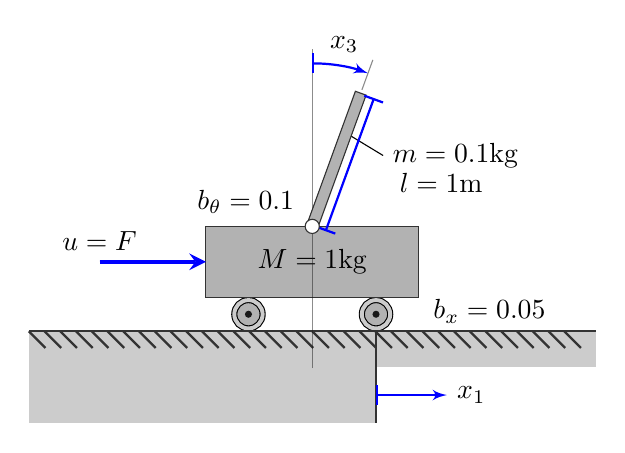
\begin{tikzpicture}[> = latex',%
	scale = 0.9]
	\tikzset{%
		interface/.style={
			% The border decoration is a path replacing decorator. 
			% For the interface style we want to draw the original path.
			% The postaction option is therefore used to ensure that the
			% border decoration is drawn *after* the original path.
			postaction={draw, decorate, decoration={border, angle=-45,
					amplitude=0.3cm, segment length=2mm}}},
		helparrow/.style={>=latex', blue, thick},
		% helparrow/.style={>=latex', draw=blue, fill=blue, very thick},
		helpline/.style={thin, black!90, opacity=0.5},
		force/.style={>=stealth, draw=blue, fill=blue, ultra thick},
	}
	\def\ground{%
		\fill [black!20] (0, 0) rectangle (49mm, -13mm);
		\fill [black!20] (49mm, 0) rectangle (80mm, -5mm);
		\draw [thick, black!80, interface] (0, 0) -- (80mm, 0);
		\draw [thick, black!80] (49mm, 0) -- +(0, -13mm);
		\draw [|->, helparrow] (49mm, -9mm) -- ++(10mm, 0) node [right] {\color{black} $x_1$ };
	}
	
	\def\cart{
		\filldraw [%thick,%
		draw = black!80,%
		fill = black!40,%
		top color = black!30,%
		bottom color = black!30,%
		% pattern=horizontal lines gray,%
		] (0,0) rectangle (30mm, 10mm);
		\node at (15mm, 5mm) {$M=1$kg};
		\draw[->, force] (-15mm, 5mm) node [above] {$u=\ensuremath{\vv{F}}$} -- (0, 5mm);
		\node at (40mm, -2mm) {$b_x = 0.05$};
	}
	
	\def\pendulum{%
		\filldraw [%thick,%
		draw = black!80,%
		% fill = black!25,%
		left color=black!30,%
		bottom color=black!30,%
		% pattern=horizontal lines gray,%
		] (-0.8mm, 0) rectangle (0.8mm, 20mm);
		\draw [|-|, helparrow] (2mm, 0mm) -- ++(0mm, 20mm);
		\node at (15mm, 12mm) {$l=1$m};
		\node at (-10mm, 0mm) {$b_\theta=0.1$}; 
	}
	
	\def\joint{%
		\filldraw [%thick,%
		draw = black!80,%
		fill = white,%
		% pattern=horizontal lines gray,%
		] (0, 0) circle (1mm);
	}
	
	\def\wheel{%
%		\fill [thin,%
%		fill = black!70,%	path fading = south
%	] (0, 0) circle (1.75mm);
%		\begin{scope}
%			\clip (0, 0) circle (1.75mm);
%			\fill [fill=black!30,] (0, -1mm) circle (2mm);
%		\end{scope}
		\fill [fill=black!30,] (0, 0mm) circle (2mm);
		\fill [fill=black!90] (0, 0) circle (0.5mm);
		\draw [thin,%
		double = black!20,%
		double distance = 0.5mm] (0, 0) circle (2mm);
	}

	\begin{scope}
		\wheel
	\end{scope}
	\begin{scope}[xshift=18mm]
		\wheel
	\end{scope}
	\begin{scope}[xshift=-31mm, yshift=-2.4mm]
		\ground
	\end{scope}
	\begin{scope}[shift = {(-6mm, 2.4mm)}]
		\cart
	\end{scope}
	\begin{scope}[shift = {(9mm, 12.4mm)}]
		\draw [helpline] (0, -20mm) -- (0, 25mm);
		\draw [helpline] (70:20.5mm) -- (70:25mm);
		\draw [|->, helparrow] (0, 23mm) 
		arc [radius=23mm, start angle=90, delta angle=-20] ;
		\node at (80:26mm) {$x_3$};
%		\draw [|->, helparrow] (0, -9mm) 
%		arc [radius=9mm, start angle=-90, delta angle=195] ;
%		\node [above right] at (50:8.5mm) {$\theta$};
		\draw [thin] (70:14mm) -- (10mm, 10mm) 
		node [right] {$m=0.1$kg};
	\end{scope}
	\begin{scope}[shift = {(9mm, 12.4mm)}, rotate=-20]
		\pendulum
	\end{scope}
	\begin{scope}[shift = {(9mm, 12.4mm)}]
		\joint
	\end{scope}
\end{tikzpicture}


%\begin{tikzpicture}[> = latex',%
%	scale = 1,%
%	text = blue]
%	\begin{scope}
%		\wheel
%	\end{scope}
%	\begin{scope}[xshift=18mm]
%		\wheel
%	\end{scope}
%	\begin{scope}[xshift=-31mm, yshift=-2.4mm]
%		\ground
%	\end{scope}
%	\begin{scope}[shift = {(-6mm, 2.4mm)}]
%		\cart
%	\end{scope}
%	\begin{scope}[shift = {(9mm, 12.4mm)}]
%		\draw [helpline] (0, -20mm) -- (0, 25mm);
%		\draw [helpline] (110:20.5mm) -- (110:25mm);
%		\draw [|->, helparrow] (0, 23mm) 
%		arc [radius=23mm, start angle=90, delta angle=20] ;
%		\node at (97:25mm) {$\theta'$};
%		\draw [|->, helparrow] (0, -9mm) 
%		arc [radius=9mm, start angle=-90, delta angle=195] ;
%		\node [above right] at (50:8.5mm) {$\theta$};
%		\draw [thin] (110:14mm) -- (-10mm, 10mm) 
%		node [left] {$m$, $I$};
%	\end{scope}
%	\begin{scope}[shift = {(9mm, 12.4mm)}, rotate=20]
%		\pendulum
%	\end{scope}
%	\begin{scope}[shift = {(9mm, 12.4mm)}]
%		\joint
%	\end{scope}
%\end{tikzpicture}\vspace{-10pt}
	\caption{Illustration of the inverted pendulum.}\label{fig:invpen}
\end{figure}

Consider the system linearized at $x_3=x_4=0$, and we sample the continuous-time linear system periodically every $0.1$ seconds. The system equation is 
\begin{align*}
	&x(k+1)=Ax(k)+Bu(k)+w(k) \\
	&=
	\begin{bmatrix}
	1&  \hspace{-4pt} 0.1  & \hspace{-4pt} -0.050  &\hspace{-4pt}  -0.002\\
	0 &  \hspace{-4pt} 1   & \hspace{-4pt}-1.012  &  \hspace{-4pt} -0.050\\
	0  &  \hspace{-4pt} 0 & \hspace{-4pt}  1.100 &  \hspace{-4pt} 0.103\\
	0   &  \hspace{-4pt} 0& \hspace{-4pt} 2.025  & \hspace{-4pt} 1.100
	\end{bmatrix}x(k)+
\begin{bmatrix}
	0.005\\
	0.102\\
	-0.005\\
	-0.103
\end{bmatrix}
u(k)+w(k),\\
%\end{align*}
%
%\begin{align*}
&y(k)=Cx(k)+v(k)+a(k)\\
&=
\begin{bmatrix}
	1& 0 &0 &0\\
	1& 0 &0 &0\\
	1& 0 &0 &0\\
	0& 0 &1 &0
\end{bmatrix}x(k)+v(k)+a(k).
\end{align*}
There are three sensors monitoring the cart position ($x_1$) and one sensor monitoring pendulum angle ($x_3$).
The noise covariances of the system satisfy $w(k) \sim {N}(0, 0.001\times I_4)$ and $v(k) \sim {N}(0, 0.001\times I_4)$.
The jordan canonical form of $A$ is 
$$
\begin{bmatrix}
	1  & 1 &  0 & 0\\
	0  & 1 & 0 &  0\\
	0  & 0 & 0.642 & 0  \\
	0  & 0 & 0 &  1.557 
\end{bmatrix},
$$
and there is a Jordan block with size $2\times 2$ and the geometric multiplicity of all the eigenvalues are 1.
According to Corollary \ref{co:sparse_obs}, the system is $2$-sparse observable and our proposed estimator secure in the presence of 1 corrupted sensor. 
The controller of the system is designed as a Linear-Quadratic Regulator (LQR), and the feedback matrix is chosen as 
$$K_{\rm lqr}=\begin{bmatrix}
	-0.604 & -1.678 & -39.514 & -9.721
 \end{bmatrix}.
$$
%
%
%In the following we perform state transformation on the origin system to better analysis the observability structure.
%There exists a invertible matrix $U$ such that 
%
%In the following, we study the following system where $\bar{C}\triangleq CU$:
%	\begin{align*}
%		\bar{x}(k+1)&=\bar{A} \bar{x}(k)+U^{-1}w(k)+U^{-1}Bu(k), \\
%		y(k)&=\bar{C} \bar{x}(k)+v(k)+a(k).
%	\end{align*}


We first illustrate the performance of estimation on close-loop system where $u(k)=-K_{\rm lqr} x(k)$.
Fig. \ref{fig:close_loop} presents the performance of the estimation of system state $x_3$ (pendulum angle). In the absence of attack, our proposed estimation substantially coincides with the Kalman estimation. The numerical difference attributes to large Gaussian noise that occurs occasionally and error in numerical calculation.
The bottom subplot represents the estimation under attack on sensor 4.
The attack $a_4(k)$ is a time-independent random value uniformly distributed on interval $(-5,5)$. As shown in the bottom of Fig \ref{fig:close_loop}, Kalman estimation (denoted as red dashed line) has larger estimation error than our proposed estimation under the attack.

%\begin{figure}[ht]
%	\centering
%	\input{est_closeloop_state3.tex}
%	\caption{Estimation of state $x_3$ (pendulum angle) in the absence and in the presence of attack. The initial state is $x(0)=[0,\ 1,\ 0,\ 1]^\top$. } \label{fig:close_loop}
%	%The optimization parameter $\gamma$ is set to be 70.
%\end{figure}

Fig. \ref{fig:MSE} illustrates the estimation mean square error (MSE) of our proposed estimator with varying $\gamma$ in the absence and in the presence of attack on sensor 3 and sensor 4. 
The attack $a_3(k)$ and $a_4(k)$ in the simulation are respectively time-independent random value uniformly distributed on interval $(-5,5)$ and interval $(-2,2)$.
The MSE of the oracle Kalman estimation, .i.e., Kalman estimation not affected by the attack, is illustrated by the red dashed line in Fig. \ref{fig:MSE}.
As shown in the figure, by properly choosing $\gamma$, the MSE of our proposed estimator is smaller than that of Kalman estimation (the red horizontal line), with the cost that MSE without attack is slightly larger. 

%\begin{figure}[ht]
%	\centering
%	\input{MSE.tex}
%	\caption{Estimation mean square error (MSE) in the absence and in the presence of attack with varying tuning parameter $\gamma$.} \label{fig:MSE}
%	%The optimization parameter $\gamma$ is set to be 70.
%\end{figure}


In order to further validate the performance of our proposed estimator in the presence of attack, the estimation is used to feed in the controller.
In Fig. \ref{fig:attack}, the red solid lines represent the pendulum angle with Kalman estimation as the feedback, i.e., when control input is $u(k)=-K_{\rm lqr} \ \hat{x}(k)$, and the red dashed lines represent the corresponding estimation $\hat{x}(k)$.
Similarly, the blue solid lines represent the pendulum angle with our proposed secure estimation as the feedback, i.e., the control input is $u(k)=-K_{\rm lqr} \ \tilde{x}(k)$, and the blue dashed lines represent the corresponding estimation $\tilde{x}(k)$.

%\begin{figure}[ht]
%	\input{est_inloop_underattack_state3.tex}
%	\caption{Performance of feedback control with our proposed estimator and Kalman estimator in the presence of attack on sensor 4. The initial state is $x(0)=[0,\ 1,\ 0,\ 1]^\top$.} \label{fig:attack} 
%	%	 The optimization parameter $\gamma$ is set to be 1.
%\end{figure}

The attack used in Fig. \ref{fig:attack} is the same as used in Fig. \ref{fig:close_loop}.
The initial state is $x(k)=[0,\ 1,\ 0,\ 1]^\top$, and the system intends to stabilize the state at zero in spite of manipulated observations and noise.
As shown in Fig. \ref{fig:attack}, the estimation error of our proposed estimator is smaller than the Kalman estimator, and the corresponding state is stabilized around zero. In contrast, the Kalman estimator is not resilient to integrity attack, and the state error from zero is larger.




%The estimation mean square error (MSE) in the absence and in the presence of attack is presented in Table \ref{tab:MSE}.
%The initial state is set to be $x(0)=\mathbf{0}$. When sensor 1 is under manipulation, the bias data is a random value uniformly distributed on interval $(-10,10)$. When sensor 4 is under manipulation, the bias data is a random value uniformly distributed on interval $(-\pi,\pi)$. The MSE of our proposed estimator is approximately the same as that of Kalman estimator in the absence of attack. In the presence of attack, the MSE of our proposed estimator is smaller.
%
%\begin{table}[h]
%	\caption{Mean square error of two estimators}\label{tab:MSE}
%	\begin{tabular}{c|c|c|c}
%	\hline 
%		Estimator & \makecell[c]{\small MSE without\\ attack} & \makecell[c]{\small MSE when \\ $\Ic=\{1\}$} &\makecell[c]{\small MSE when \\ $\Ic=\{4\}$} \\
%	\hline 
%		\makecell[c]{Kalman\\ estimator} & 0.0121 & 0.6652 & 2.8834 \\ 
%		\hline
%		\makecell[c]{Our proposed\\ estimator}  & 0.0122 & 0.4927 & 0.5025 \\
%		\hline 
%	\end{tabular}
%\end{table}





\section{Conclusion}\label{sec:conclusion}
This paper considers LTI system with Gaussian noise against malicious attack on a subset of sensors. 
We improve upon the previous work by reducing the computation complexity in the designing phase while remaining low computation complexity for online estimation, under the assumption that all the geometric multiplicities of eigenvalues of $A$ are $1$.
To achieve this, we prove that the span of the rows of $G_i$ is equivalent to the observable space, based on which the canonical form $H_i$ is designed. The proposed estimator is formulated as a convex optimization problem based on $H_i$. We further prove that the proposed estimation is secure if the system is $2p$-sparse observable, which is easily checked due to the simple form of $H_i$. Moreover, in the absence of attack, the proposed estimation coincides with Kalman estimation for certain probability, which can be adjusted by tuning parameter $\gamma$ to balance between the performance with and without attack.
The condition of $2p$-sparse observable is necessary for secure state reconstruction \cite{ShoukryTAC2016} and our proposed estimator achieves this fundamental limit with low computation complexity.
%For general $A$ without the geometric multiplicity assumption, calculating sparse observability index is NP-hard. 

%In previous works, we proposed a information fusion scheme by decomposing Kalman estimation into the linear combination of local estimates. 
%However, whether this estimator is resilient cannot be validated within polynomial time.
%In this paper, by introducing the assumption that all the eigenvalues of $A$ have geometric multiplicity 1, we prove that the structure of matrix $G_i$ is closely related to observability matrix of system $(A,C_i)$. This result enables us to design a secure estimator that is resilient to $p$ compromised sensors as long as the system is $2p$-sparse observable and this can be further relaxed to $2p$-sparse detectable. Moreover, the estimate coincides to Kalman estimate for certain probability in the absence of attack.  we design an algorithm that can compute sparse observability index in polynomial time. 
%However, when the geometric multiplicity is greater than 1, Lemma \ref{lm:span} no long holds and there are instances where $\rs(G_i)\neq \rs{O_i}$. We are currently investigating the solution in this case. Nevertheless, by decomposing the $n$ dimensional space into multiple orthogonal generalized eigenspaces, the problem of checking sparse observability can be significantly simplified. 


%%%%%%%%%%%%%%%%%%%%%%%%%%%%%%%%%%%%%%%%%%%%%%%%%%%%%%%%%%%%%%%%%%%%%%%%%%%%%%%%

\appendix
%\subsection{Proof of Lemma }
%\begin{proof}
%	Since according to \cite{garone_cdc16}, $\rs{G_i}\subseteq {\rm span}\{C_iA^k|=0,\cdots,n-1\}$, one obtains that, for each $i\in\Rc$, there exists a group of basis vector $\{\alpha_{i,1},\cdots,\alpha_{i,n}\}$ such that 
%	\begin{equation*}
%		content...
%	\end{equation*} 
%\end{proof}
\subsection{Proof of Theorem \ref{th:main}}\label{ap:th_main}
\begin{proof}
	%	Define $\tilde{M}\triangleq\tilde{P}\tilde{W}\tilde{P}^\top$.
	Consider the KKT condition of problem (\ref{pb:lasso}) and one obtains $\tilde{M}^{-1}\mu=\gamma\cdot \sgn(\nu)$,	
	%	 denote the dual variables for equation constraints as $\lambda=[\lambda_1^{\top},\cdots,\lambda_m^{\top}]^{\top}\in \Cb^{mn\times 1}$. 	
	%	
	%	\begin{align}
	%		\tilde{M}^{-1}\mu - \lambda &= \mathbf{0} \label{eq:KKT1}\\
	%		H^{\top}\lambda &= \mathbf{0} \label{eq:KKT2} \\
	%		\gamma \cdot  \sgn(\nu) - \lambda &= \mathbf{0} \label{eq:KKT3} \\
	%		\Yc - H \tilde{x} - \mu - \nu &= \mathbf{0}  \label{eq:KKT4}
	%	\end{align}
	where $\sgn(\cdot)$ is the subgradient of $\|\cdot\|_1$, i.e., for the $i$-th entry:
	\begin{align*}
		[\sgn(\nu)]_i=\partial |[\nu]_i|=
		\left\{
		\begin{array}{cc}
			-1 ,& \ [\nu]_i<0 \\
			1 , &\ [\nu]_i>0  \\
			\{x|-1\leq x\leq 1\},& \ [\nu]_i=0 
		\end{array}
		\right. .
	\end{align*}
	The time index $(k)$ is omitted for notation conciseness.
	Therefore, one obtains $\mu=\gamma\cdot \tilde{M}\sgn(\nu)$ and thus
	$\|\mu\|_\ift\leq \gamma \left\|\tilde{M}\right\|_\ift$.
	We proceed to prove that solution $\tilde{x}$ is bounded.
	Notice that we are optimizing the following problem %(\ref{pb:LASSO_free}) 
	\begin{align*}%\label{pb:LASSO_free}
		\min _{\mu,\tilde{x}} \frac{1}{2} \mu^{\top} \tilde{W}^{-1} \mu+\gamma\left\|\Yc-\mu-H \tilde{x}\right\|_1 ,
	\end{align*}
	and suppose $\mu$ has taken the value of optimal solution $\mu^*$.
	It is sufficient to minimize the following:
	\begin{align}\label{pb:1-norm_min}
		\min_{\tilde{x}} \sum_{i\in\Rc} \left\|P_i \zeta_{i}-\mu^*_{i}- H\tilde{x} \right\|_1  .
	\end{align}
	Notice that $P_i \zeta_{i}$ and $\mu^*_{i}$ are fixed known values.
	Define $\xi_i\triangleq P_i \zeta_{i}-\mu^*_{i} $ and recall $[\cdot]_j$ is the $j$-th entry of a vector. The objective function in (\ref{pb:1-norm_min}) can be written as
	\begin{align}
		&\sum_{i\in\Rc}\sum_{j=1}^{n} \left| [\xi_i]_j -[H \tilde{x}]_j \right| 
		=\sum_{j=1}^{n}\sum_{i\in\Sc_j} \left| [\xi_i]_j -[\tilde{x}]_j \right| . \label{eq:solve_for_median}
	\end{align}
	where $|\cdot|$ means absolute value and $\Sc_j$ is defined in \eqref{eq:def_Oc}. 
	For each state index $j$, the minimizer $[\tilde{x}]_j$ of objective (\ref{eq:solve_for_median}) could be explicitly written as the median of all $[\xi_i]_j$ among $i\in\Sc_j$.
	
	Before proving that $[\tilde{x}]_j$ is bounded, let us define the following operator: $f_{i}: R \times R \times \cdots \times R \rightarrow R,$ such that $f_{i}\left(\alpha_{1}, \ldots, \alpha_{m}\right)$ equals to the $i$-th smallest element in the set $\left\{\alpha_{1}, \ldots, \alpha_{m}\right\} .$ For even number $m$, we further define 
	$$f_{\frac{m+1}{2}} = \left(f_{\frac{m}{2}} + f_{\frac{m}{2}+1}\right)/2.$$ 
	Thus, $f_{(m+1)/2}\left(\alpha_{1}, \ldots, \alpha_{m}\right)$ is the median number of set $\left\{\alpha_{1}, \ldots, \alpha_{m}\right\}$ and the solution to problem \eqref{pb:1-norm_min} is
	\begin{align*}
		[\tilde{x}]_j = f_{(m+1)/2}\left([\xi_i]_j, i\in\Sc_j\right).
	\end{align*}
	Define the number of honest sensors and compromised sensors (w.r.t. compromised set $\Ic$) that can observe state $j$ as:
	\begin{align*}
		h_j(\Ic)\triangleq |\Sc_j\cap \Ic^c|, \
		c_j(\Ic)\triangleq |\Sc_j\cap \Ic|.
	\end{align*}
	We have the following lemma quantifying the property of $h_j(\Ic)$ and $c_j(\Ic)$.  
	\begin{lemma}\label{lm:cj<hj}
		If the system is $2p$-sparse observable, for any $\Ic$ with $|\Ic|=p$, we have $c_j(\Ic)<h_j(\Ic)$ for all $j\in\{1,2,\cdots,n\}$.
	\end{lemma}
	\begin{proof}
		We prove by contradiction. Supposing that there exists $j^*$ and $\Ic^*$ with $|\Ic^*|=p$ such that $ c_{j^*}(\Ic^*)\geq h_{j^*}(\Ic^*)$, then
		$h_{j^*}(\Ic^*)\leq c_{j^*}(\Ic^*)\leq |\Ic^*|=p$. Noticing that $c_j(\Ic)+h_j(\Ic)=|\Sc_j|$ holds for all $\Ic$, we have $|\Sc_{j^*}|\leq 2p$. 
		Define set $\Ac$ that satisfy $\Ac\supseteq\Sc_{j^*}$ and $|\Ac|=2p$.
		According to the definition of $\Sc_{j^*}$, there exists no sensor in set $\Rc\setminus \Ac$ who can observe state $j^*$, i.e.,
		\begin{equation*}
			e_{j^*}\notin \rs(O_i),\ \forall i\in\Rc\setminus \Ac.
		\end{equation*}
		As a result, system $(A,C_{\Rc\setminus\Ac})$ is not $2p$-sparse observable according to Definition \ref{df:sparse_obs}, which leads to contradiction.
	\end{proof}
	Recalling the definition of $\zeta^{\re}_{i}$ in \eqref{eq:def_zetare}, we define $\xi^{\re}_{i}$ correspondingly as $\xi^\re_i\triangleq P_i\zeta^\re_{i}-\mu^*_{i} $.
	Based on the definition of $h_j,c_j$ ($\Ic$ is omitted for notation simplicity), we have
	\begin{align}	
		f_{(h_j-c_j)}\left([\xi^\re_i]_j, i\in\Sc_j\right) &\leq
		f_{(m+1)/2}\left([\xi_i]_j, i\in\Sc_j\right), \label{eq:x_u_leftbound}\\
		f_{(m+1)/2}\left([\xi_i]_j, i\in\Sc_j\right)&\leq 
		f_{2c_j}\left([\xi^\re_i]_j, i\in\Sc_j\right) .  \label{eq:x_u_rightbound}
	\end{align}
	According to Lemma \ref{lm:cj<hj}, $h_j-c_j>0$ and $2c_j<h_j+c_j=|\Sc_j|$.
	As a result, according to (\ref{eq:x_u_leftbound}) and (\ref{eq:x_u_rightbound}), one obtains
	\begin{align}\label{eq:med_bound}
		\min \left\{ [\xi^\re_i]_j, i\in\Sc_j \right\}\leq [\tilde{x}]_j\leq \max \left\{ [\xi^\re_i]_j, i\in\Sc_j \right\}.
	\end{align}
	Consider the following optimization problem without attack:
	\begin{align*}
		&\underset{{x}^o(k), \mu^o(k),\nu^o(k)}{\operatorname{minimize}}\quad \frac{1}{2} (\mu^o(k))^\top \tilde{M}^{-1} \mu^o(k) + \gamma_0\|\nu^o(k)\|_1 \\
		&\ \text{ subject to }\quad \
		\tilde{P}\zeta^\re(k)=H {x}^o(k) +\mu^o(k)+\nu^o(k). 
	\end{align*}
	Denote the solution as $x^o, \mu^o, \nu^o$. 
	According to Theorem \ref{th:no_attack}, by choosing 
	$$\gamma_0\triangleq \left\| \tilde{M}^{-1}\left(I-GF\right) \epsilon^\re(k) \right\|_{\infty} ,$$
	the solution coincides with Kalman estimation, i.e., $x^o(k)=\hat{x}(k)$.
	Similar to previous analysis, the solution $x^o(k)$ satisfies 
	\begin{align}\label{eq:normal_solution}
		[x^o]_j=f_{(m+1)/2}\left( [P_i\zeta_{i}^\re-\mu^o_i]_j, i\in\Sc_j \right).
	\end{align}
	Combining \eqref{eq:med_bound} and \eqref{eq:normal_solution} leads to that, for every $j\in\{1,2,\cdots,n\}$,
	\begin{align*}
		&\left|[\tilde{x}]_j-[x^o]_j\right| =\left|[\tilde{x}]_j-[\hat{x}]_j\right|\\
		\leq &
		\max_{i_1,i_2\in \Sc_j} \left| \left[P_{i_1} \zeta^\re_{i_1}(k)\right]_j- \left[P_{i_2} \zeta^\re_{i_2}(k)\right]_j \right| 
		+ \|\mu^*\|_\infty+ \|\mu^o\|_\infty\\
		\leq& \max_{i_1,i_2\in \Sc_j} \left| \left[P_{i_1} \zeta^\re_{i_1}(k)\right]_j- \left[P_{i_2} \zeta^\re_{i_2}(k)\right]_j \right| +(\gamma+\gamma_0)\|\tilde{M}\|_\ift.
	\end{align*}
Recall that $P_i\epsilon_{i}(k)=P_i \zeta_i (k)-H_ix(k)$. Since for all $i_1,i_2\in \Sc_j$, one obtains $H_{i_1}x(k)=H_{i_2}x(k),\forall k\in\Zb^+$. Thus, we have
\begin{align*}
&\max_{i_1,i_2\in \Sc_j} \left| \left[P_{i_1} \zeta^\re_{i_1}(k)\right]_j- \left[P_{i_2} \zeta^\re_{i_2}(k)\right]_j \right| \\
=&\max_{i_1,i_2\in \Sc_j} \left| \left[P_{i_1} \epsilon^\re_{i_1}(k)\right]_j- \left[P_{i_2} \epsilon^\re_{i_2}(k)\right]_j \right| ,
\end{align*}
whose variance is uniformly bounded for all $k$ according to Lemma \ref{lm:epsilon}. Similarly, $\gamma^o$ is also uniformly bounded for all $k$. Therefore, our estimation $\tilde{x}$ is secure according to Definition \ref{def:resi}.
\end{proof}


	
%	\section*{ACKNOWLEDGMENT}

%%%%%%%%%%%%%%%%%%%%%%%%%%%%%%%%%%%%%%%%%%%%%%%%%%%%%%%%%%%%%%%%%%%%%%%%%%%%%%%%

%	\end{thebibliography}
\bibliographystyle{IEEEtran}
%	\bibliographystyle{plain}
\bibliography{ref_zishuo}

\addtolength{\textheight}{-12cm}   % This command serves to balance the column lengths
% on the last page of the document manually. It shortens
% the textheight of the last page by a suitable amount.
% This command does not take effect until the next page
% so it should come on the page before the last. Make
% sure that you do not shorten the textheight too much.


\end{document}
